\section{基于IMU预积分技术的VISLAM}

接下来重点介绍IMU预积分技术\citep{forster2017manifold}。与普通基于IMU积分的VISLAM系统不同,IMU预积分使用了更精确的相对运动模型。将IMU观测模型包含三个部分:相对旋转、相对速度、相对平移,可以认为它们是仅关于偏移量的函数。使用以下算法进行IMU预积分,假设需要对$t_i$和$t_j$之间IMU读数进行积分(假设相邻两帧IMU之间时间间隔相同,即$\Delta t_{i,i+1} = \Delta t_{i+1,i+2} = \cdots = \Delta t_{j-1,j} = \Delta t$):

\begin{equation}
\begin{aligned}
\mathrm{R}_j &= \mathrm{R}_i \prod_{k=i}^{j-1}
                \exp\left(
                    (\tilde{\bm\omega}_k - \bm{b}_k^g - \bm{n}_k^g) \Delta t
                \right) \\
\bm{v}_j &= \bm{v}_i + \bm{g} \Delta t_{ij} + \sum_{k=i}^{j-1}
\mathrm{R}_k (\tilde{\bm{a}}_k - \bm{b}_k^a - \bm{n}_k^a) \Delta t \\
\bm{p}_j &= \bm{p}_i + \sum_{k=i}^{j-1}
                \left[
                    \bm{v}_k \Delta t +
                    \tfrac{1}{2}\bm{g}\Delta t^2 +
                    \tfrac{1}{2}\mathrm{R}_k
                    (\tilde{\bm a}_k - \bm{b}_k^a - \bm{n}_k^a) \Delta t^2
                \right]
    \end{aligned}
\end{equation}

传统的VISLAM中,通常将连续关键帧之间的一系列IMU读数进行积分,得到相对的状态变化$\Delta\bm X$,然后加上前一个关键帧的状态$\bm{X}_i$,得到下一个关键帧的状态$\bm{X}_j$,同时计算出累积的协方差,作为下一个关键帧的先验估计,参与到视觉的优化中去。这样做的缺陷就是,积分项$\Delta\bm X$实际上会随着偏移量的更新而改变,除非在每一轮优化迭代时重新积分计算新的$\Delta\bm X$,否则IMU积分项的误差会一直存在。

按照如下方式定义状态$\bm{X}_i$和$\bm{X}_j$之间的相对状态变化$\Delta\bm X$:

\begin{equation}
\begin{aligned}
    \Delta\mathrm{R}_{ij}
  &\doteq \mathrm{R}_i^\top \mathrm{R}_j
  = \prod_{k=i}^{j-1}
  \exp\left(
      (\tilde{\bm \omega}_k - \bm{b}_k^g - \bm{n}_k^g) \Delta t
  \right) \\
  %
  \Delta\bm{v}_{ij}
  &\doteq \mathrm{R}_i^\top (\bm{v}_j - \bm{v}_i - \bm{g} \Delta t_{ij})
  = \sum_{k=i}^{j-1}
  \Delta\mathrm{R}_{ik}
  (\tilde{\bm a}_k - \bm{b}_k^a - \bm{n}_k^a) \Delta t \\
  %
  \Delta\bm{p}_{ij}
  &\doteq \mathrm{R}_i^\top
  \left(
      \bm{p}_j - \bm{p}_i -
      \bm{v}_i \Delta t_{ij} -
      \tfrac{1}{2} \bm{g} \Delta t_{ij}^2
  \right) \\
  &=           \sum_{k=i}^{j-1}
  \left[
      \Delta\bm{v}_{ik} \Delta t +
      \tfrac{1}{2} \Delta\mathrm{R}_{ik}
      (\tilde{\bm a}_k - \bm{b}_k^a - \bm{n}_k^a) \Delta t^2
  \right]
\end{aligned}\label{eq:raw_int}
\end{equation}

每一轮优化迭代过后,使用一阶的线性方法对$\Delta\mathrm{R}_{ij}$,$\Delta\bm{p}_{ij}$,$\Delta\bm{v}_{ij}$这三个量进行更新,这样就使得在状态变量随着优化在更新的时候,状态的观测也在不断地向着更准确的方向更新,使得整个观测模型更加精准,这也是预积分工作的最主要贡献。

\section{预积分项的误差模型}

传统的迭代式IMU积分也可以通过不断地重新积分来不断地使观测模型变精准,但是每次重新积分的计算代价太大,一般实际应用中意义不大。而预积分的基本操作就是首先假设两帧之间的偏移量为定值,即$\bm{b}_i = \bm{b}_{i+1} = \cdots = \bm{b}_{j-1}$,然后将式\eqref{eq:raw_int}的普通IMU积分项认为是与预积分项-白噪声带来的扰动量之和:

\begin{equation}
\begin{aligned}
    \Delta\mathrm{R}_{ij} &\doteq
        \Delta\tilde{\mathrm R}_{ij}(\bm{b}^g_i) \exp(-\delta\bm\phi_{ij}) \\
    \Delta\bm{v}_{ij} &\doteq
        \Delta\tilde{\bm v}_{ij}(\bm{b}^g_i, \bm{b}^a_i) - \delta\bm{v}_{ij} \\
    \Delta\bm{p}_{ij} &\doteq
        \Delta\tilde{\bm p}_{ij}(\bm{b}^g_i, \bm{b}^a_i) - \delta\bm{p}_{ij}
\end{aligned}
\end{equation}

最终可以得到IMU预积分项$\left[\Delta\tilde{\mathrm R}_{ij},\Delta\tilde{\bm v}_{ij},\Delta\tilde{\bm p}_{ij}\right]$和预积分的误差项$\bm{n}_{ij} \doteq \left[\delta\bm\phi_{ij},\delta\bm{v}_{ij},\delta\bm{p}_{ij}\right]$,并且认为这个$9$维的误差也是符合均值为零的高斯分布的。记它的协方差为$\Sigma_{ij}$,即$\bm{n}_{ij} \sim \mathcal{N}\left(\bm{0},\Sigma_{ij}\right)$。而这个协方差,显然是在预积分的过程中通过IMU读数的白噪声累积得来的。因此需要在预积分的过程中根据白噪声的协方差$\bm{n} \doteq \left[\bm{n}^g,\bm{n}^a\right] \sim \mathcal{N}(\bm{0},\mathrm\Sigma_{\bm{n}})$同时也完成白噪声的传递。限于篇幅,白噪声的传递的推导,这里不再给出。

\section{偏移量的线性修正}

上面提到,预积分技术使用线性的方法将每轮迭代时偏移量增量更新到预积分项中去,作为其修正。因此需要先将偏移量写成一个偏移量初值加迭代小增量的形式:
\begin{equation}
\begin{aligned}
    \hat{\bm b}^g_i &= \bar{\bm b}^g_i + \delta\bm{b}^g_i \\
    \hat{\bm b}^a_i &= \bar{\bm b}^a_i + \delta\bm{b}^a_i
\end{aligned}
\end{equation}

记$\Delta\bar{\mathrm R}_{ij}\doteq\Delta\tilde{\mathrm R}(\bar{\bm b}^g_i), \Delta\bar{\bm v}_{ij}\doteq\Delta\tilde{\bm v}_{ij}(\bar{\bm b}^g_i,\bar{\bm b}^a_i), \Delta\bar{\bm p}_{ij}\doteq\Delta\tilde{\bm p}_{ij}(\bar{\bm b}^g_i,\bar{\bm b}^a_i)$,按如下方式进行线性修正:
\begin{equation}
\begin{aligned}
    \Delta\tilde{\mathrm R}_{ij}(\hat{\bm b}_i^g)
    &\doteq \Delta\tilde{\mathrm R}_{ij}(\bar{\bm b}^g_i + \delta\bm{b}^g_i)
    \simeq \Delta\bar{\mathrm R}_{ij}
    \exp\left(
      \tfrac{\partial\Delta\bar{\mathrm R}_{ij}}{\partial\bm{b}^g_i}
      \delta\bm{b}^g_i
    \right) \\
    %
    \Delta\tilde{\bm v}_{ij}(\hat{\bm b}^g_i,\hat{\bm b}^a_i)
    &\doteq \Delta\tilde{\bm v}_{ij}(
    \bar{\bm b}^g_i + \delta\bm{b}^g_i,
    \bar{\bm b}^a_i + \delta\bm{b}^a_i)
    \simeq \Delta\bar{\bm v}_{ij} +
    \tfrac{\partial\Delta\bar{\bm v}_{ij}}{\partial\bm{b}^g_i}
    \delta\bm{b}^g_i +
    \tfrac{\partial\Delta\bar{\bm v}_{ij}}{\partial\bm{b}^a_i}
    \delta\bm{b}^a_i \\
    %
    \Delta\tilde{\bm p}_{ij}(\hat{\bm b}^g_i,\hat{\bm b}^a_i)
    &\doteq \Delta\bar{\bm p}_{ij}(
    \bar{\bm b}^g_i + \delta\bm{b}^g_i,
    \bar{\bm b}^a_i + \delta\bm{b}^a_i)
    \simeq \Delta\bar{\bm p}_{ij} +
    \tfrac{\partial\Delta\bar{\bm p}_{ij}}{\partial\bm{b}^g_i}
    \delta\bm{b}^g_i +
    \tfrac{\partial\Delta\bar{\bm p}_{ij}}{\partial\bm{b}^a_i}
    \delta\bm{b}^a_i
\end{aligned}
\label{eq:bias_upd}
\end{equation}

这样,在每轮优化迭代的时候,需要同时使用式\eqref{eq:bias_upd},将新的偏移量更新到IMU预积分结果里。不过,当必要的时候,比如偏移量的增量非常大,那么线性更新可能精度也是不够的,此时还是可以采用重新积分的方式去更新预积分项,以减少误差累积。

\section{非线性优化}

基于迭代式IMU积分的VISLAM中,IMU项参与优化的方式一般比较直接——使用IMU积分得到状态先验,再和视觉观测融合,反复迭代。例如OKVIS中的非线性优化(如图~\ref{fig:okvis}是OKVIS优化的因子图)。

\begin{figure}[htb!]
    \centering
    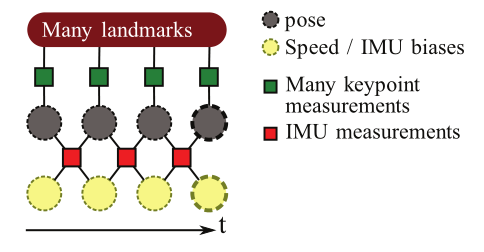
\includegraphics[width=.5\textwidth]{./figs/okvis.png}
    \caption{OKVIS因子图示例图\citep{leutenegger2015keyframe}}
    \label{fig:okvis}
\end{figure}

和大部分的SLAM系统一样,IMU预积分技术的后端优化也是基于非线性最小二乘。它的能量函数同样包括基本的视觉观测项和IMU预积分项(见图\ref{fig:preint}),形式上没有区别,区别仅在IMU部分的能量:
\begin{equation}\label{eq:gtsam_res}
    \bm{\mathcal X}^\star =
        \arg\mathop{\min}_{\bm{\mathcal X}}
        \sum_{i,j}\left\| \bm{r}_{\mathcal{I}_{ij}} \right\|^2_{\mathrm\Sigma_{ij}} +
        \sum_{i} \sum_{l} \left\| \bm{r}_{\mathcal{C}_{il}} \right\|^2_{\mathrm\Sigma_{C}}
\end{equation}

\begin{figure}[htb!]
    \centering
    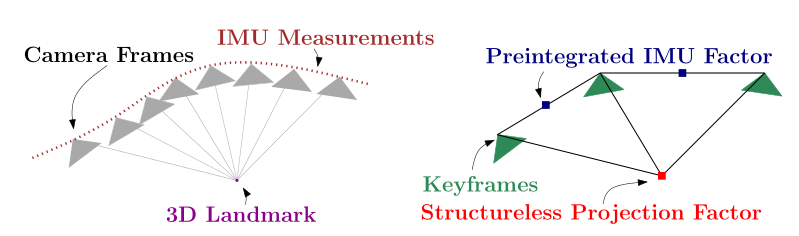
\includegraphics[width=.6\textwidth]{./figs/preint.png}
    \caption{IMU预积分因子图示例\citep{forster2017manifold}}
    \label{fig:preint}
\end{figure}

其中$\bm{r}_{\mathcal{C}_{il}}$是关于状态$i$和路标点$l$的视觉部分目标函数,这一部分的定义和大部分SLAM系统一致。$\bm{r}_{\mathcal{I}_{ij}}$则与MSCKF、OKVIS等系统不同,是关于相邻状态$i$和$j$的IMU预积分目标函数。在IMU预积分技术中,这一项被认为是仅和状态$i$的偏移量相关的函数:$\Delta\tilde{\mathrm R}_{ij}(\bm{b}^g_i)$、$\Delta\tilde{\bm v}_{ij}(\bm{b}^g_i, \bm{b}^a_i)$和$\Delta\tilde{\bm p}_{ij}(\bm{b}^g_i, \bm{b}^a_i)$。前面已经给出了IMU预积分项的误差模型,因此可以很容易地写出IMU预积分项的目标函数:

\begin{equation}
\begin{aligned}
  \bm{r}_{\Delta\mathrm{R}}
    &\doteq
      \log\left(
        \left(
          \Delta\bar{\mathrm R}_{ij}
          \exp\left(
            \tfrac{\partial\Delta\bar{\mathrm R}_{ij}}{\partial\bm{b}^g_i}
            \delta\bm{b}^g_i\right)
        \right) \mathrm{R}^\top_i \mathrm{R}_j
      \right) \\
  \bm{r}_{\Delta\bm{v}}
    &\doteq
      \mathrm{R}^\top_i(\bm{v}_j - \bm{v}_i - \bm{g}\Delta t_{ij}) -
      \left[
        \Delta\bar{\bm v}_{ij} +
        \tfrac{\partial\Delta\bar{\bm v}_{ij}}{\partial\bm{b}^g_i}
        \delta\bm{b}^g_i +
        \tfrac{\partial\Delta\bar{\bm v}_{ij}}{\partial\bm{b}^a_i}
        \delta\bm{b}^a_i
      \right] \\
  \bm{r}_{\Delta\bm{p}}
    &\doteq
      \mathrm{R}^\top_i(
        \bm{p}_j - \bm{p}_i -
        \bm{v}_i \Delta t_{ij} -
        \tfrac{1}{2}\bm{g}\Delta t^2_{ij}) -
      \left[
        \Delta\bar{\bm p}_{ij} +
        \tfrac{\partial\Delta\bar{\bm p}_{ij}}{\partial\bm{b}^g_i}
        \delta\bm{b}^g_i +
        \tfrac{\partial\Delta\bar{\bm p}_{ij}}{\partial\bm{b}^a_i}
        \delta\bm{b}^a_i \right]
\end{aligned}
\end{equation}
